% AUTO-GENERATED by writeup/make_dh_causal_standalone_tex.py
% Build: pdflatex -interaction=nonstopmode dh_causal_standalone.tex
\documentclass{article}
\usepackage[T1]{fontenc}
\usepackage{lmodern}
\usepackage[landscape,margin=0.48in]{geometry}
\usepackage{booktabs}
\usepackage{amsmath}
\usepackage{graphicx}
\pagestyle{empty}
\begin{document}
\begin{center}
{\large\bfseries 0DTE delta-hedged ATM straddles, 11:00 entry held till close/\mbox{15:30}}\\[0.5ex]
\small Every day sells the nearest-OTM straddle at 11:00 and delta-hedges to 16:00. At 15:30 each forecast model decides on its own whether to buy the straddle back: exit the short if \emph{that} model's $s>0$ (its realized variance forecast above implied); otherwise cash-settle.
\\[0.9ex]
% AUTO-GENERATED by writeup/make_dh_causal_standalone_tex.py
\begingroup\small\setlength{\tabcolsep}{3.6pt}
\begin{tabular}{lrrrrrrrrrrrr}
\toprule
& $n$ & mean & std & min & max & $t$ & Sharpe$_{\mathrm{ann}}$ & Sharpe$^{\times}_{\mathrm{ann}}$ & MaxDD & MaxDD$^{\times}$ & $n_{\mathrm{exit}}$ & \%exit \\
\midrule
hold through cash-settle & 865 & 0.103 & 0.388 & -2.30 & 0.87 & 7.78 & 4.20 & 3.58 & -3.48 & -3.80 & 0 & 0.0 \\
\addlinespace
\multicolumn{13}{l}{exit if $s>0$} \\
\quad baseline (HAR + calendar OLS) & 865 & 0.102 & 0.377 & -2.30 & 0.87 & 7.96 & 4.30 & 3.66 & -3.21 & -3.57 & 286 & 33.1 \\
\quad block-diagonal ridge & 865 & 0.104 & 0.365 & -2.30 & 0.87 & 8.36 & 4.51 & 3.85 & -3.84 & -4.25 & 346 & 40.0 \\
\quad block-diagonal ridge, without the FOMC columns & 865 & 0.106 & 0.357 & -2.30 & 0.87 & 8.74 & 4.72 & 4.05 & -3.81 & -4.21 & 355 & 41.0 \\
\quad LightGBM & 865 & 0.108 & 0.370 & -2.30 & 0.87 & 8.62 & 4.65 & 4.00 & -3.38 & -3.78 & 289 & 33.4 \\
\quad XGBoost & 865 & 0.108 & 0.370 & -2.30 & 0.87 & 8.56 & 4.62 & 3.97 & -3.75 & -4.15 & 278 & 32.1 \\
\quad lasso (causally tuned) & 865 & 0.107 & 0.366 & -2.30 & 0.87 & 8.64 & 4.66 & 4.01 & -3.53 & -3.94 & 321 & 37.1 \\
\quad lasso (fixed 1e-4) & 865 & 0.103 & 0.365 & -2.30 & 0.87 & 8.33 & 4.50 & 3.84 & -3.81 & -4.21 & 358 & 41.4 \\
\quad elastic net (causally tuned) & 865 & 0.105 & 0.367 & -2.30 & 0.87 & 8.38 & 4.52 & 3.87 & -3.85 & -4.25 & 307 & 35.5 \\
\bottomrule
\end{tabular}
\endgroup

\end{center}
\vspace{0.7em}
\noindent\small\textbf{Delta hedge.} (1)~Sell the nearest-OTM call and put at 11:00; those strikes stay unchanged. (2)~Every later 30-minute stamp until 15:30, read the vendor spot and vendor hourly IV at that stamp. Total vol is that IV times the square root of hours remaining to 16:00. Straddle delta is Black--76 call delta plus put delta (interest rate zero, forward = spot). Because the straddle is short, hold plus-delta of the index. Stock P\&L over the next half hour is delta times the spot change. (3)~At 15:30, if \emph{that row's} model has $s>0$, buy the straddle back at the Black--76 mark and close the stock. If not, cash-settle versus the GSPC close (last stock step uses that close versus the 15:30 spot). No look-ahead: the entry uses only the 11:00 quote; each rebalance uses only the quote at that stamp.
\vspace{0.35em}
\begin{center}
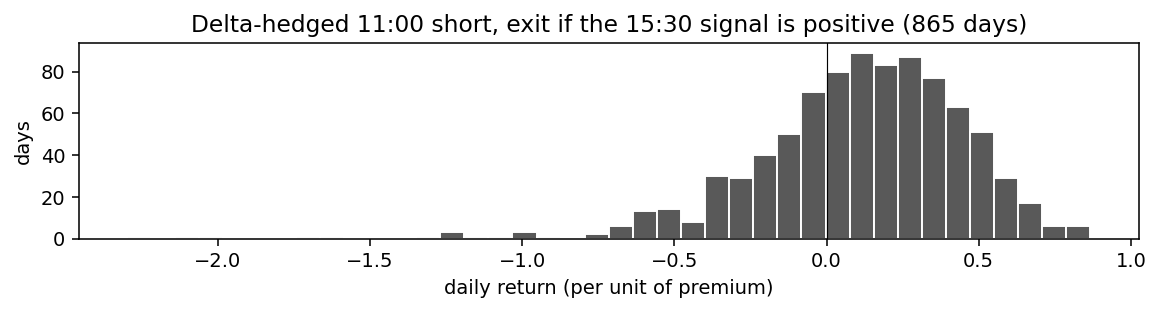
\includegraphics[width=0.76\textwidth]{../results/atm_straddle_intraday_holdclose/proposals/26/dh_causal_hists.png}\\[0.25ex]
\small Daily return of the 11:00 short; 15:30 exit uses the block-diagonal ridge $s$.
\end{center}
\par\vspace{0.35em}
\noindent\small One expiration day is one return. \mbox{Sharpe$_{\mathrm{ann}}=(\mathrm{mean}/\mathrm{std})\times\sqrt{252}$}. $t$-stat is $\sqrt{n}\cdot\mathrm{mean}/\mathrm{std}$. Every day enters at 11:00. Each model only decides whether to exit at 15:30. $n_{\mathrm{exit}}$ is days that model buys the straddle back. Sharpe$^{\times}_{\mathrm{ann}}$ is the same book at the crossed spread: sell the 11:00 straddle at the bid, then cash-settle or buy back at the 15:30 mark; P\&L is still divided by the midpoint premium. MaxDD is the worst peak-to-trough decline of the cumulative sum of the daily returns, in date order, one unit a day (summed, not compounded), signed and in units of entry premium like min; MaxDD$^{\times}$ is the same at the crossed spread.
\end{document}
